\subsection{Criteria Pollutants}%
\label{sub:criteria_pollutants}

Criteria pollutants are a group of six chemical species, commonly found
mixed in air, that constitute a serious hazard for human, animal, and
general environment health. These pollutants were defined in 1970,
through the Clean Air Act in the United States, but have since been
widely adopted. These six pollutants are:
\begin{enumerate}
    \item \glsxtrlong{PM};
    \item \glsxtrlong{o3};
    \item \glsxtrlong{co};
    \item \glsxtrlong{so2};
    \item \glsxtrlong{no2};
    \item Lead (Pb);
\end{enumerate}

They are collectively addressed as criteria pollutants, solely because
environmental agencies around the world have since been using them, and
their atmospheric concentrations as criteria for setting standards. Of
the 6 criteria pollutants, 4 are of direct importance for this
dissertation, as \gls{DOAS} can be used to measure and quantify them.
They are \gls{PM}, \gls{o3}, \gls{so2} and \gls{no2}. This section aims
to provide a brief presentation of these four species.

\subsubsection{\glsxtrlong{PM}}%
\label{ssub:pm}

Particles are aggregates of many molecules, that can be similar of
different. There are several processes in which particles can be formed,
and they can be chemically active or, for instance, act as surfaces on
which trace gases may condense. The chemical composition of a particle
is immensely variable, and it can even be difficult to determine, since
one particle sample (usually collected over a period of some hours) can
have thousands of species, namely hydrocarbons. One interesting aspect
of \gls{PM} is that its volume distribution is bimodal, having two clear
maxima below 1$\mu$m and another around 10$\mu$m. The reason for this
separation is the way in which the particles were formed. Coagulations
and condensation tend to form the smaller particles, while the larger
peak is comprised mostly of crustal (as in from the Earth's crust)
and sea solids, together with some smaller aggregated particles --
smaller particles that have adhered onto one another.
Figure~\ref{fig:particle_distribution} illustrates this bimodal
distribution and the responsible formation phenomena.

\begin{figure}[htpb]
    \centering
    % left, bottom, right, top
    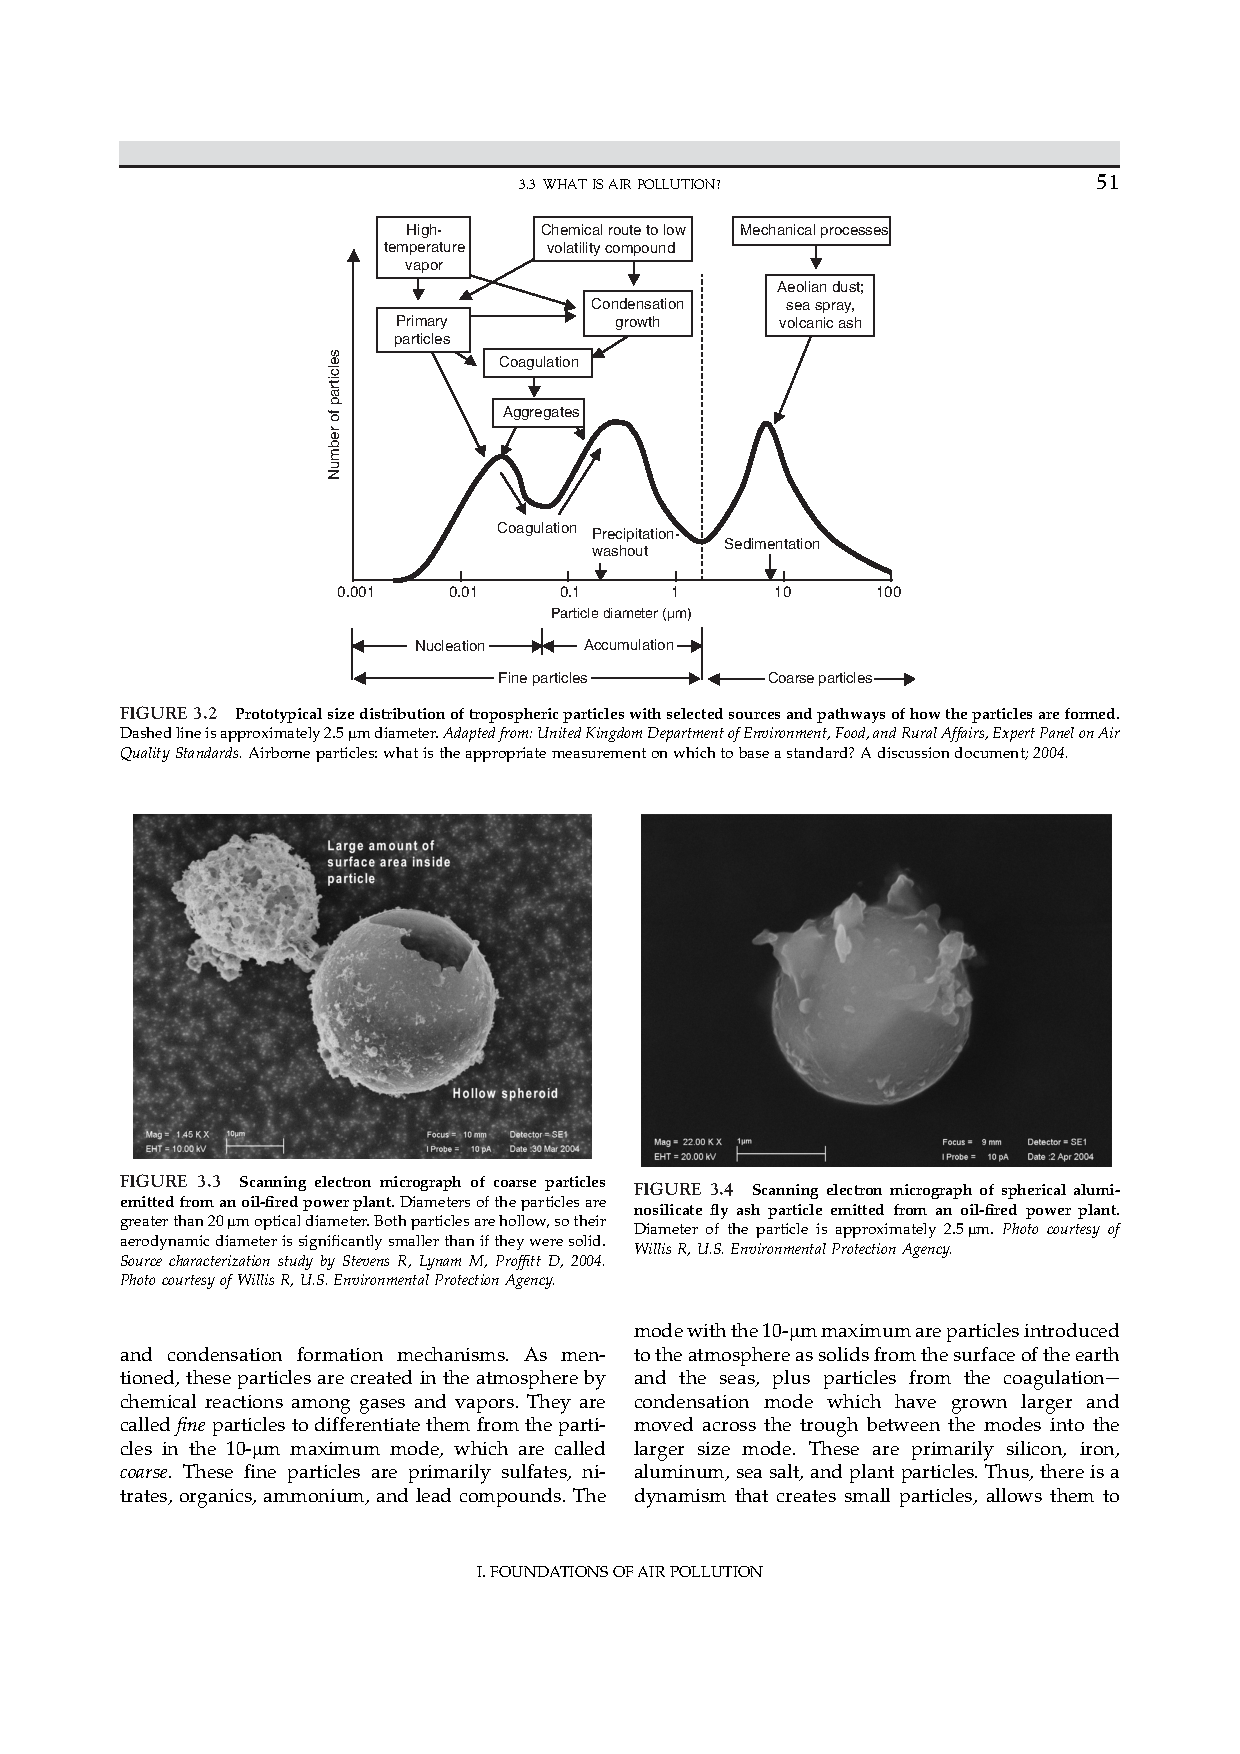
\includegraphics[clip,%
    trim=5.5cm 19.1cm 5.5cm 3.5cm,%
    width=.8\textwidth]{img/pdf/vallero_bimodal_particles.pdf}
    \caption{Bimodal distribution for particle volume and the phenomena
    that lead to their formation~\cite{Vallero2014}}
    \label{fig:particle_distribution}
\end{figure}


\subsubsection{Tropospheric \glsxtrlong{o3}}%
\label{ssub:tropospheric_o3}

Ozone is one of the most important trace gases in the atmosphere, in
functional terms.  The \gls{o3} concentration in lower troposphere has
had a sharp rise in recent decades, which indicates that this rise is
anthropogenic in nature~\cite{Bourdeau}.  In the last \gls{EEA} reports,
European concentrations of \gls{o3} have remained approximately stable
and just above the \gls{WHO}-set limit for the protection of human
life~\cite{EEA2016, Guerreiro2019}. In both reports, the \gls{EEA}
states that although ozone precursor concentrations have been steadily
declining, concentrations for \gls{o3} remain the same, although the
amplitude of peak events is shown to be decreasing (see
Figure~\ref{fig:o3peaksvsmean})

\begin{figure}[htpb]
    \centering
    % left, bottom, right, top
    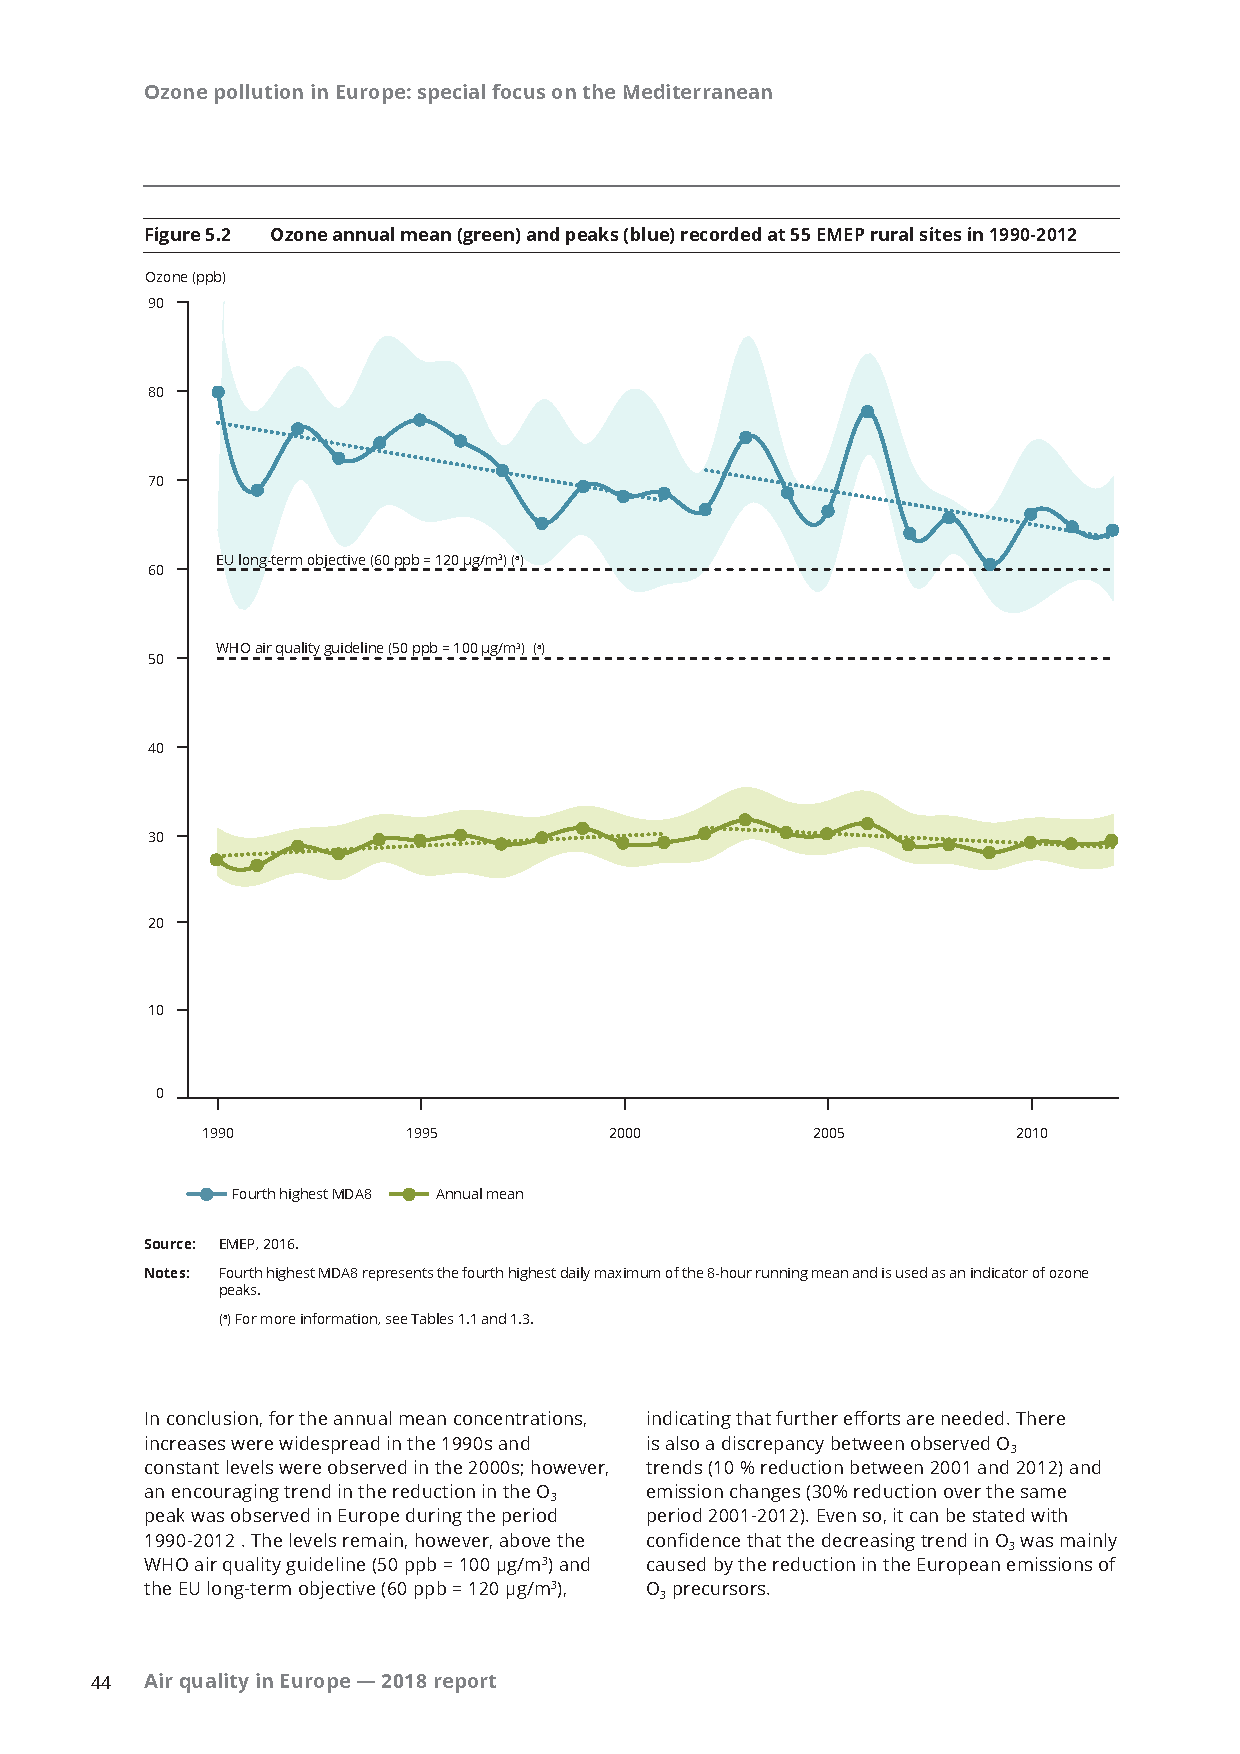
\includegraphics[clip,%
    trim=2.2cm 10.2cm 2cm 4.4cm,%
    width=.8\textwidth]{img/pdf/eea2018_ozone_peaks.pdf}
    \caption{Ozone mean and peaks in European rural sites. Peaks are
    plotted blue, mean is plotted green. Note the decrease in peak
    concentration and the steadyness of the mean signal.}
    \label{fig:o3peaksvsmean}
\end{figure}

Ozone formation in the lower atmosphere is also interesting. While other
pollutants are directly emitted by its sources, \gls{o3} is a secondary
pollutant, which means that it is formed through chemical reactions that
its precursors endure. With the exception of \gls{VOC}, these precursors
are results from human activity. There innumerable pathways for ozone
formation. Table~\ref{tab:ozoneformation} summarizes the main avenues.

\begin{table}
    \centering
    \caption{Main avenues for the formation of ozone in the troposphere.}
    \label{tab:ozoneformation}
\end{table}


\subsubsection{\glsxtrlong{so2}}%
\label{ssub:so2}

Nitrogen, Sulphur, Phosphorous and Potassium are very familiar to those
accustomed to dealing with plant life. For plants, these 4 chemicals
are. Their life depends on them. However, from an \gls{AP} point of
view, sulphur and nitrogen compounds are common issues and have to be
addressed separately. We will deal with \gls{no2} in
Section~\ref{ssub:no2}. Sulphur compounds are released into the
atmosphere primarily through anthropogenic activities (for instance,
diesel-powered engines), although marine biogenic gases represent a
significant proportion of the emitted sulphuric species.

These compounds can be released in reduced and oxidised forms, although
reduced forms are generally oxidised onto \gls{so2}. \gls{so2} has many
complex atmospheric chemical reactions, but proceeds to the sulphate ion
through at least three pathways. If given enough time, sulphur oxidises
into SO\textsubscript{4}\textsuperscript{-}, usually forming sulphuric
acid. This reacts readily with ammonia in the atmosphere, and produces
ammonium sulphates that, together with their precursor sulphuric acid,
are readily dissolved in water~\cite{Bourdeau}.

\subsubsection{\glsxtrlong{no2}}%
\label{ssub:no2}

\gls{no2} is the most important atmospheric trace gas as far as this
thesis is concerned, for reasons that will become clear in
Section~\ref{sec:experiment}. Nitrogen oxides are toxic, but that is not
the only reason why they are problematic. In fact, they are one of the
main precursors of tropospheric ozone, namely through photolysis, as
described in Equation~\ref{eq:no2_photolysis}.

\begin{align}
    \label{eq:no2_photolysis}
    NO_2 + h\nu \rightarrow NO + O
    O + O_2 + M \rightarrow O_3
\end{align}

$M$, in the case of Equation~\ref{eq:no2_photolysis}, is any third body
that absorbs excess vibration energy and can stabilise the newly formed
molecule. But \gls{o3} can go on to react with \gls{no} and regenerate
\gls{no2} and \gls{o2}, as in Equation~\ref{eq:no2_formation}.

\begin{equation}
    \label{eq:no2_formation}
    O_3 + NO \rightarrow NO_2 + O_2
\end{equation}

Now, these reactions and several others that involve nitrogen species
occur whether there is pollution or not,  which results in an
equilibrium \gls{o3} concentration of 30 ppb. In a polluted atmosphere,
say by \gls{ice}, this balance is destroyed. Fossil fuel combustion
increases \gls{nox} concentration, but also concentrations of
hydrocarbons through incomplete combustion. This means that in addition
to the balanced atmospheric reactions of nitrogen species, we now have
to consider the oxidation of these long hydrocarbon chains, which
produce \gls{no2} without destroying \gls{o3}, thus upsetting the
initial balace.
